\begin{figure}[ht]
\begin{center}
 \begin{ccTexOnly}
   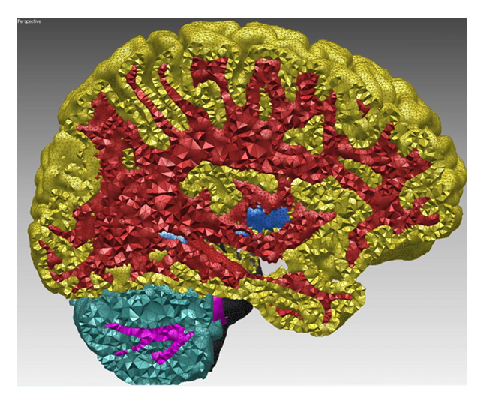
\includegraphics[height=9cm]{Mesh_3/pictures/multilabel_mesher}
 \end{ccTexOnly}
 \begin{ccHtmlOnly}
   <img border="0" src="./pictures/multilabel_mesher.jpg"><br/>
 \end{ccHtmlOnly}
 \caption{Cut-view of a multi-domain 3D mesh generated from a segmented image.}
  \label{figure:multilabel_mesher}
\end{center}
\end{figure}

\section{Introduction}
\label{Mesh_3_section_intro}

This package is devoted to the generation of  isotropic simplicial
meshes discretizing 3D domains.
%The main component of this package is a function which 
%generates 3D  simplicial meshes.
The domain to be meshed is a region of 3D space that has to be bounded.
The region may be connected or  composed of multiple components
and/or subdivided in several subdomains. 
%  We refer to the domain as a multi-domain
% when the different subdomains need to be
% distinguished from each other.

Boundary and subdivision surfaces  are either
smooth or piecewise smooth surfaces, formed with planar or curved surface patches.
Surfaces may exhibit $1$-dimensional features (e.g. crease edges)
and $0$-dimensional features (e.g. singular points as corners
 tips, cusps or darts), that have to be fairly
approximated in the mesh.

% Generally speaking, we may think of the input domain as 
% a $3$-dimensional complex whose faces of dimension 3, 2, 1 and 0
% are called respectively subdomain, surface patches, curve segment 
% and corners.


The output mesh is a 3-dimensional triangulation, 
including subcomplexes that approximate each input domain feature: subdomain,
boundary surface patch or input domain feature with dimension $0$ or $1$.
Thus,  the output mesh includes  a 3D submesh covering each  subdomain, 
a surface mesh approximating  each boundary or subdividing
surface patch, a polyline approximation for  each 
$1$-dimensional feature and 
of course  a vertex on each  corner.


 The main entry points of the package are
two global  functions that respectively generate
and refine such meshes.
The mesh generator is customized to output a mesh
that fits as much as possible the user needs,
for instance in terms of  sizing field 
or with respect to some user customized quality criteria.


The  meshing engine used in this mesh generator
is  based on  Delaunay refinement~\cite{c-gqmgc-93, r-draq2d-95, s-tmgdr-98}.
It uses the notion of restricted Delaunay triangulation
 to approximate $1$-dimensional curve segments and   surface patches~\cite{cgal:bo-pgsms-05}.
Before the refinement, a mechanism of protecting balls is set up on $1$-dimensional features, if any,
 to ensure a fair representation
of those features in the mesh, and also to guarantee the termination of the refinement process,
whatever may be the input geometry, in particular whatever small angles
the boundary and subdivision surface patches may form~\cite{cgal:cdl-pdma-07,cgal:cdr-drpsc-07}.
The Delaunay refinement is followed by a mesh  optimization phase
to remove slivers and provide a good quality mesh.
 




\subsubsection{Input domain}

The  domain to be meshed is assumed to be bounded
 and  representable as a pure
3D complex. A 3D complex is a set of faces with dimension~0,
1, 2  and~3  such that
all faces are pairwise interior disjoint, 
and the boundary of each face of the complex is the union of faces
of the complex.
The 3D complex is pure, meaning that each face is included in a face of dimension 3,
so that the complex is entirely described by the set of its 3D faces and their subfaces.
However the 3D complex needs not be connected.
The set of faces with dimension lower or equal than~2 forms a 2D
subcomplex which needs not be manifold, neither pure, nor connected:
some 3D faces may have dangling 2D or 1D faces in their boundary faces.

In the rest of the documentation, we will refer to the
input 3D complex as  the input domain. The faces of the input domain 
with dimension $0$, $1$, $2$ and $3$ are called respectively
{\em corners},  {\em curve segments}, {\em surface patches} and {\em subdomains}
to clearly distinguish them from the faces of the mesh
that are called vertices, edges, facets and cells.

Note that the input complex faces are not required to be linear nor smooth.
Surface patches, for instance, may be smooth surface patches, 
or portions of surface meshes with boundaries.
Curve segments may be  for instance straight segments, curved segments
or polylines. Each of those features will be accurately represented in the final mesh.



The $0$ and $1$-dimensional features of the input domain are usually singular  points
of the subdomain boundaries, however this is not required. Furthermore those features
are not required to cover all the subdomains  boundaries singularities
 but only those that need to be accurately represented in the final mesh.
In the following, we say that a domain has {\em features} when it has $0$ and
$1$-dimensional features that need to be accurately represented in the mesh,
and we call those features {\em exposed features}.
Therefore, a domain may be without features either because all boundary surface patches
are smooth closed surfaces, or simply because the curves  joining  different surface patches
and the singularities of those  patches need not be accurately approximated
in the final mesh.

Note also that input complex faces are not  required to be connected.
Faces of the input domain are identified by  indexes.
If a subdomain is not connected, its different components receive the same index.
Likewise different surface patches, segment curves or corners may share the same index.
Each connected component of a feature  will be accurately represented
in the final mesh.
Note however that the occurrence of multiply connected faces in the
input complex may affect the relevance of internal topological checks
performed by the mesh generator.  Also the mesh generator
will not be able to apply  different meshing criteria, e.g. different
sizing field, for the different connected components of a single feature. 

The domain is input to the mesh generation function,
as a domain class, often called  the  oracle,
that provides predicates and constructors related to the domain,
the subdomains, the boundary surface patches
and  also the $0$ and $1$-dimensional exposed features, if any.
Mainly, the oracle provides  a predicate to test
if  a given query point belongs 
to the domain or not
and  to find in which subdomain it lies in the affirmative case.
The domain class also provides predicates  and constructors to test the intersection of a query line segment
with the boundary  surface patches and to build some intersection points if any.
Lastly, if the input domain includes $1$-dimensional exposed features, the domain class
provides a way to construct sample points on these features.

The current implementation provides  classes to represent
domains bounded by isosurfaces of implicit functions, polyhedral domains
and domains defined through 3D labeled images. 
Currently,  $1$-dimensional features may be defined as segments and polyline segments.

% The resulting mesh is output as a subcomplex of a 3D triangulation,
% in the form of a class providing various output iterators
% on mesh elements.

\subsubsection{Output mesh}

The resulting mesh is output as a subcomplex of a 3D Delaunay triangulation,
in a class  providing various iterators
on mesh elements.

 The 3D triangulation provides approximations of the
subdomains, surface patches and curve segments
and corners, according to the restricted
Delaunay triangulation paradigm. This means that each subdomain
 is approximated by the union of  the tetrahedral cells
 whose circumcenters are located inside the domain
(or subdomain). 
Each surface patch  is approximated 
by the union of   the Delaunay mesh  facets whose dual Voronoi edges intersect the surface patch.
Such mesh  facets are called {\em surface facets}  in the following. 
The $1$-dimensional exposed features are approximated by  sequences of  mesh edges
and  the $0$-dimensional exposed features are represented by mesh vertices.



\subsubsection{Delaunay Refinement}
\label{introsec:param}

The mesh generation algorithm is  mainly a Delaunay refinement process.
The Delaunay refinement is 
preceded by a protecting phase to ensure an accurate representation
of $1$-dimensional features if any,
and  followed by an optimization  phase to achieve a good quality mesh.

%  which is currently implemented
% using the  sliver exudation approach~\cite{cgal:cdeft-slive-00}.
The   Delaunay refinement process is driven by criteria
concerning either the size and shape of  mesh cells 
and surface facets.
%i.e., the facets of the mesh whose role is to approximate surface patches.
The refinement process terminates when there are
no more mesh cells or  surface facets violating the  criteria.


The criteria are designed to achieve a nice spread of the mesh vertices
while ensuring the termination of the refinement process.
Those criteria  may  be  somehow tuned  to  the user needs 
to achieve for instance the respect of a sizing field by mesh elements,
some topological conditions on the representation of boundary surfaces  in the mesh,
and/or some error bound for the approximation of boundary surfaces.
To some extend, the user may  tune the Delaunay refinement 
to a prescribed trade-off
between mesh quality and  mesh density. 
The mesh density refers to the number of mesh vertices and cells,
i.e. to the complexity of the mesh.
The mesh quality referred to here is  measured by the radius edge
ratio of surface facets end mesh cells, where the radius edge ratio of
a simplex (triangle or tetrahedron) is the
the ratio between its circumradius  and  its shortest edge.

 
\subsubsection{Protection of $0$- and $1$-dimensional exposed features}

If the domain description includes $0$ dimensional features,
the corresponding  points are inserted into the Delaunay triangulation 
from the start.

If the domain has $1$-dimensional exposed features,
the method of protecting balls~\cite{cgal:cdr-drpsc-07, cgal:cdl-pdma-07}
is used to achieve an accurate representation of those features in the mesh
and to guarantee that the refinement process terminates
whatever may be the dihedral  angles formed by input  surface patches incident to a
given $1$-feature or the  angles formed by two $1$-features incident to a  $0$-feature.

According to this method,  the $1$-dimensional features are 
sampled with points and covered by protecting balls centered on the sample points,
 in such a way that~:\\
-no three balls intersect \\
-no pair of balls centered on different $1$-features intersect.

The  triangulation embedding the mesh is in fact 
a weighted Delaunay triangulation, and the  triangulation 
is initialized by the insertion of all the protecting
balls, regarded as weighted points.
The Delaunay refinement process
is then launched  as before except that refinement points
are no longer circumcenters but are 
 weighted circumcenters.
All Steiner vertices inserted by the refinement process are given a zero weight.

The method guarantees:\\
1) that each segment joining
two successive centers on a $1$-dimensional feature will stay in the triangulation,
thus ensuring an accurate approximation of  the $1$-dimensional features. \\
2) that the refinement process will never try to insert a refinement point in the union of the
protecting balls, which ensures the termination of the refinement process.



\subsubsection{Optimization phase}

Any tetrahedron that is quasi degenerate has a big radius edge ratio except
those belonging to the family of slivers.  A sliver is easily obtained 
as the convex hull of 4 points close to the equatorial circle of a 3D
ball and roughly equally spread along this circle.
The Delaunay refinement tracks tetrahedra with big radius edge ratio 
and therefore eliminates all kinds of 
 badly shaped tetrahedra except slivers.

Therefore, at the end of the refinement process,
some sliver shaped tetrahedra may occur in the mesh.
The optimization phase aims at eliminating slivers.

The optimization phase is a succession of optimization processes,
including possibly a Lloyd smoothing, an odt-smoothing,
a perturber and an exuder.

The  Lloyd and odt-smoother are global optimizers
 moving the  mesh vertices to  minimize  
a   mesh energy.   Those optimizers are described respectively in 
\cite{cgal:dfg-cvtaa-99t, cgal:dw-tmgob-02} and  in \cite{cgal::c-mssbo-04,cgal:acyd-vtm-05}.
In both cases the mesh energy
is  the \ccc{L1}  error  resulting from the interpolation 
of the function $f(x) =x^2$ by a  piecewise linear function.
In the case of the Lloyd smoother,
the interpolation  is  linear in each Voronoi cell of the set of  mesh vertices.
In the case of the odt-smoother,  the interpolation is linear in each cell 
of the Delaunay triangulation of the  mesh vertices,
hence the name odt which is an  abbreviation for ``optimal Delaunay triangulation''.


\begin{figure}[ht]
\begin{center}
 \begin{ccTexOnly}
   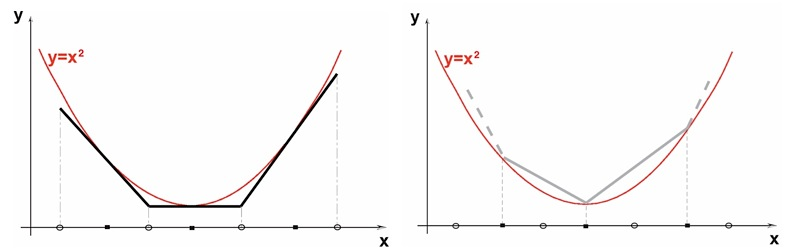
\includegraphics[width=\textwidth]{Mesh_3/pictures/paraboloid}
 \end{ccTexOnly}
 \begin{ccHtmlOnly}
   <img border="0" src="./pictures/paraboloid.jpg"><br/>
 \end{ccHtmlOnly}
 \caption{The one dimensional illustration of the mesh energy minimized by Lloyd (right)  and ODT (left) smoothers.}
  \label{figure:ODT_Lloyd_energy}
\end{center}
\end{figure}

 The Lloyd optimizer is known to be blind to the occurrence of slivers in the mesh 
while the odt-smoother tends to chase them out.
Both of them are global optimizers, 
meaning that they try to improve
the whole mesh rather than focusing on the worst elements. However, both  are empirically known
to be very efficient as a preliminary step of optimization, as they tend to enhance the
efficiency of the perturber and/or exuder applied next, see Figure~\ref{figure:optimization}

The perturber and  the exuder focus on improving the worst mesh elements.
The perturber~\cite{cgal:tsa-ps3dd-09} improves the meshes by local changes
in  the vertices positions
aiming to make sliver disappear. The exuder~\cite{cgal:cdeft-slive-00}
chases the remaining slivers by
re-weighting mesh vertices with  optimal weights.

Each optimization process can be activated or not, and tuned
according to the user requirements and the available time.
By default, only the perturber and  the exuder are activated.

Optimization processes are designed to improve mesh quality. However, beware that such an improvement
is obtained by perturbing mesh vertices and modifying the mesh connectivity which has an impact
on the strict compliance to the refinement criteria. Though a strict compliance to mesh criteria
is granted at the end of the Delaunay refinement, this may  no longer be true after
some optimization processes. Also beware that the default behavior does involve some
optimization processes.


\begin{figure}[ht]
\begin{center}
 \begin{ccTexOnly}
   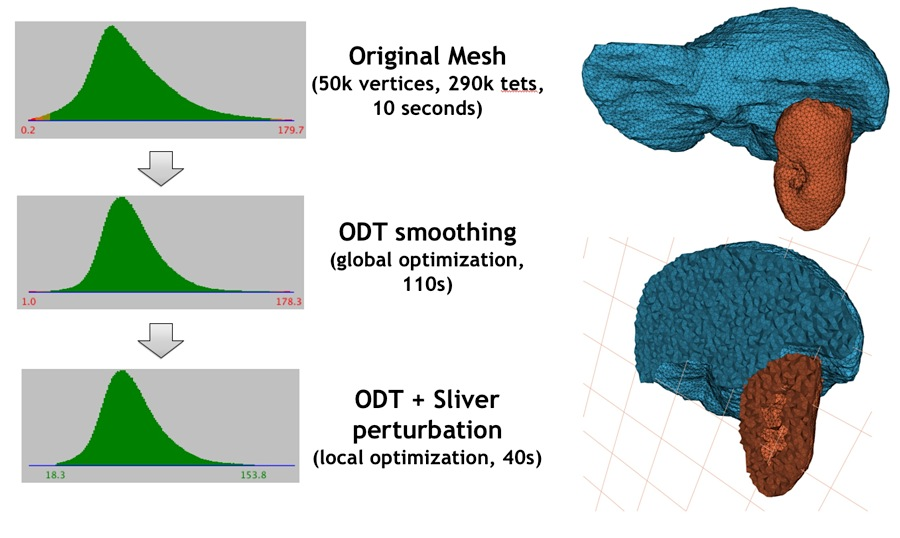
\includegraphics[width=\textwidth]{Mesh_3/pictures/optimization}
 \end{ccTexOnly}
 \begin{ccHtmlOnly}
   <img border="0" src="./pictures/optimization.jpg"><br/>
 \end{ccHtmlOnly}
 \caption{Compared effect of a global optimizer and the perturber.
The left part shows the distribution of dihedral angles of mesh cells,
right after Delaunay refinement (top), after some ODT smoothing (middle) 
and after perturbation (bottom). The numbers under the histograms give
the measure in degrees of the
smallest and biggest dihedral angles in the  mesh.}
  \label{figure:optimization}
\end{center}
\end{figure}


\section{Interface}
\label{Mesh_3_section_interface}

\subsubsection{The global functions}
A 3D mesh generation  process is launched through a call
 to   one of the two following functions:
 
\ccGlobalFunction{
  template <class C3T3,
  class MeshDomain_3,
  class MeshCriteria>
  C3T3 make_mesh_3(MeshDomain_3 domain, 
                   MeshCriteria criteria,
                   parameters::internal::Features_options features = parameters::features(domain),
                   parameters::internal::Lloyd_options lloyd = parameters::no_lloyd(),
                   parameters::internal::Odt_options odt = parameters::no_odt(),
                   parameters::internal::Perturb_options perturb = parameters::perturb(),
                   parameters::internal::Exude_options exude = parameters::exude()); }{}
             

\ccGlobalFunction{
  template <class C3T3,
  class MeshDomain_3,
  class MeshCriteria>
  void refine_mesh_3(C3T3& c3t3,
                     MeshDomain_3 domain,
                     MeshCriteria criteria,
                     parameters::internal::Lloyd_options lloyd = parameters::no_lloyd(),
                     parameters::internal::Odt_options odt = parameters::no_odt(),
                     parameters::internal::Perturb_options perturb = parameters::perturb(),
                     parameters::internal::Exude_options exude = parameters::exude()); }{}


The function \ccc{make_mesh_3} generates from scratch a mesh
of the input domain, while
the function \ccc{refine_mesh_3} refines
an existing mesh of the input domain. Note that as the protection
of 0- and 1-dimensional features does not rely on Delaunay 
refinement, the function \ccc{refine_mesh_3} has no parameter
to preserve features.


\subsubsection{The data structure}
The template parameter \ccc{C3T3} is required to be a model of
the concept 
\ccc{MeshComplex_3InTriangulation_3}, a data structure devised to
represent a three dimensional complex embedded in a 3D
triangulation. In both functions,  an instance  of type \ccc{C3T3} is used to maintain the current
approximating simplicial mesh 
and to represent the final  3D mesh at the end
of the procedure.
The type \ccc{C3T3} is   required to provide a nested type
\ccc{C3T3::Triangulation_3} for the 3D triangulation
embedding the mesh. 
This triangulation is required to be a \ccc{CGAL::Regular_triangulation_3}.
with  vertex and cell base classes  that are    respectively  models of the
concepts \ccc{MeshVertexBase_3} and \ccc{MeshCellBase_3}.

\subsubsection{The domain oracle and the features parameter}
The template parameter \ccc{MeshDomain_3} is required to be a model of
the concept  \ccc{MeshDomain_3}. The argument \ccc{domain} of type
\ccc{MeshDomain_3}
 is the sole link through which the domain
to be discretized is known  by the mesh generation algorithm. 

This concept  provides, among others,
  member functions to test whether or not
a query segment intersects boundary surfaces,
and to compute an intersection point  in the affirmative.
The \ccc{MeshDomain_3} concept adds  member functions 
which given a query point tell whether the point lies
inside or outside the domain and in which subdomain the point lies
if inside.

If the domain description includes $0$ and $1$-dimensional features
that have to be accurately represented in the final mesh,
the  template parameter \ccc{MeshDomain_3} is required to be 
of a model of the refined concept
\ccc{MeshDomainWithFeatures_3}. Mainly 
the concept \ccc{MeshDomainWithFeatures_3}  provides
 the incidence
graph of $0$, $1$ and $2$-dimensional features,
and  a member function to construct
sample points on curve segments.

Using the parameter of type \ccc{Features}, the user
whose domain is a model of \ccc{MeshDomainWithFeatures_3} 
can choose to have the corners and curve segments of the domain
represented in the mesh or not.
% The interface also provides a parameter \ccc{features} that allows
% the user to specify if $0$ and $1$-dimensional features have actually to be
% taken into account or not
%  when the domain is a model of \ccc{MeshDomainWithFeatures_3}.
The type \ccc{Features} of this parameter is an internal undescribed type.
The library provides functions to construct appropriate values of that type.
\begin{itemize}
\item \ccc{parameters::features(domain)} sets \ccc{features} according to the domain,
  i.e. $0$ and $1$-dimensional features are taken into account if \ccc{domain} is a
\ccc{MeshDomainWithFeatures_3} 
\item \ccc{parameters::no_features()} prevents the representation 
of $0$ and $1$-dimensional features in the mesh. This is useful to get a smooth and rough approximation
of a domain with features.
\end{itemize}

% There are compatibility requirements between the template parameter 
% \ccc{C3T3} and \ccc{MeshDomain}.
% The nested types \ccc{MeshDomain::Subdomain_index},
% and \ccc{MeshDomain::Index} 
% have to be convertible respectively
% to the nested types \ccc{C3T3::Triangulation::Cell::Subdomain_index}
% and  \ccc{C3T3::Triangulation::Vertex::Index}.

\subsubsection{The meshing criteria}
The template parameter \ccc{MeshCriteria} must be a model of the concept
\ccc{MeshCriteria_3}, or a model of  the refined concept \ccc{MeshCriteriaWithFeatures_3}
if the domain has exposed features.
The argument of
type \ccc{MeshCriteria} passed to the mesh generator specifies the
size and shape requirements for the tetrahedra in the mesh
and for the triangles in the boundary surface mesh. These criteria
condition the rules that drive the refinement process.  At the end 
of the refinement process, mesh elements satisfy the criteria.
This may not be strictly true anymore after the optimization phase, but this
last phase is devised to only improve the mesh quality.

The criteria  for surface facets are governed by the four following
parameters:
% \subsection{Parameters}
% \label{introsec:param}
%
% Some parameters are given to the refinement process to customize
% the generated mesh. Actually, each parameter correspond to a criteria
% that must be fullfilled by either each surface facet (if it is a
% \emph{surface facet parameter}) or each tetrahedron (if it is a
% \emph{cell parameter}). The mesh generation process ends when there is
% no more \emph{bad facet} or \emph{bad cell} given these criteria.
%
% In this package, we provide the following criteria. Note that each criteria may be
% deactivated by setting it to $0$.
%
%\subsubsection{Surface facet Parameters}
\begin{itemize}
\item \emph{\ccc{facet_angle}.} This parameter controls the shape of  
  surface facets. Actually, it is a lower bound for the angle (in degree) of
   surface  facets. When  boundary surfaces are smooth,  the termination  of the meshing process is
guaranteed  if the angular bound is at most 30
  degrees. 
\item \emph{\ccc{facet_size}.} This parameter controls the size of surface facets. 
 Actually, each surface facet has 
a surface Delaunay ball which is a ball circumscribing the surface facet and
  centered on the surface patch. The parameter \ccc{facet_size} is
  either a constant or a spatially variable scalar field,  providing an 
  upper bound for the radii of surface Delaunay balls.
 \item \emph{\ccc{facet_distance}.}  This parameter controls the approximation error of boundary and subdivision surfaces.
 Actually,   it is
  either a constant or a spatially variable scalar field. It
 provides  an upper bound for the distance between the circumcenter
 of a surface facet and the center of a surface Delaunay ball of this facet.
 \item \emph{\ccc{facet_topology}.} This parameters controls the set of topological constraints
	which have to be verified by each surface facet. By default, each vertex of a surface
	facet has to be located on a surface patch, on a curve segment, or on a corner. It can
	also be set to check whether the three vertices of a surface facet belongs to the same
	surface patch. This has to be done cautiously, as such a criteria needs that each surface
	patches intersection is an input 1-dimensional feature.
\end{itemize}

%\subsubsection{Cell Parameters}
The criteria for mesh cells are governed by two parameters:
\begin{itemize}
\item \emph{\ccc{cell_radius_edge_ratio}.}   This parameter controls the
  shape of mesh cells (but can't filter slivers, as we discussed earlier).
 Actually, it is an upper bound for the ratio
 between the circumradius of a 
   mesh tetrahedron and its shortest edge.
There is a theoretical bound for this parameter:
the Delaunay refinement process is guaranteed to terminate
for values of \ccc{cell_radius_edge_ratio}  bigger than 2.
%\item \emph{the radius bound:}
\item \emph{\ccc{cell_size}.}
This parameter controls the size of mesh tetrahedra.
It is either a scalar or a spatially variable scalar field.
  It provides an upper bound on the circumradii of the
 mesh tetrahedra. 
\end{itemize}

Figure~\ref{figure:parameters} shows how the mesh generation process
behaves with respect to these parameters.

\begin{figure}[ht]
\begin{center}
 \begin{ccTexOnly}
   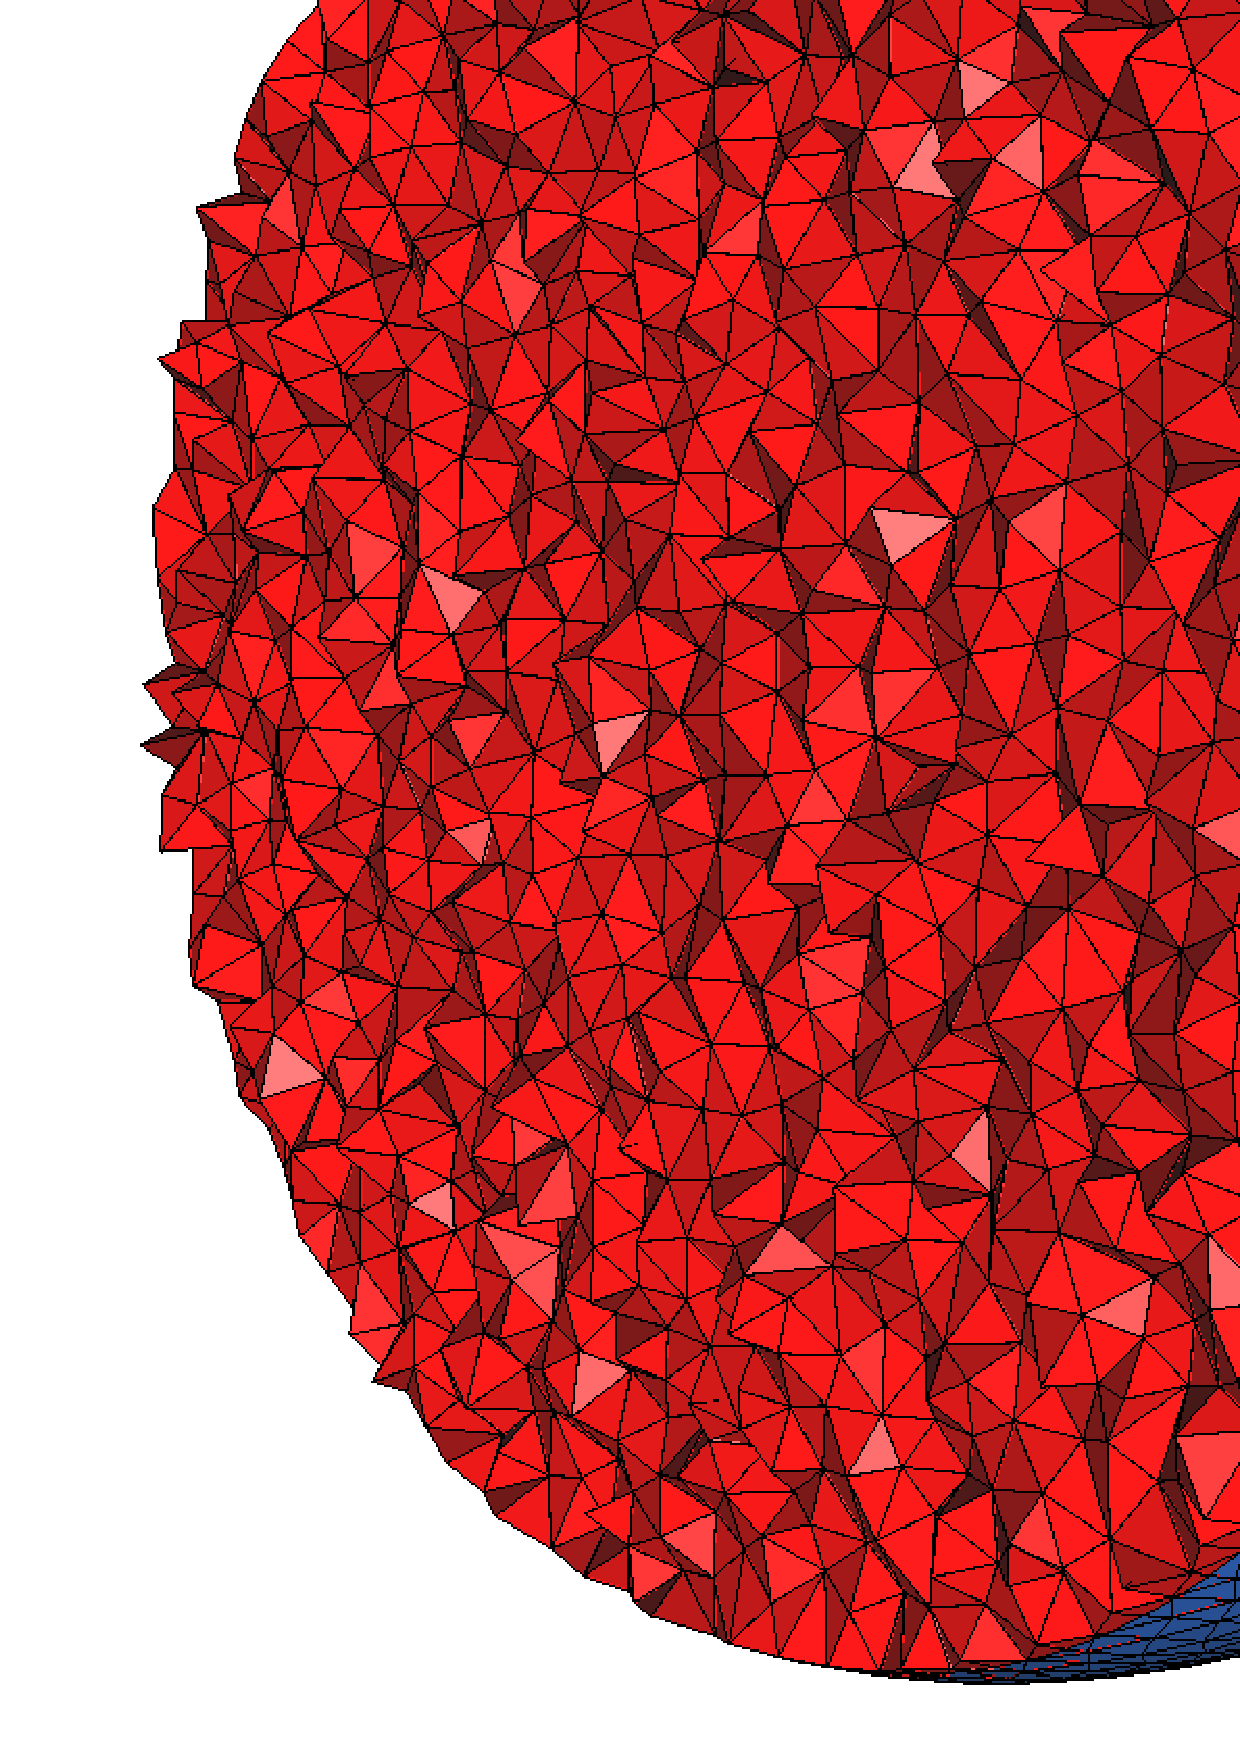
\includegraphics[height=5cm]{Mesh_3/pictures/implicit_domain}

   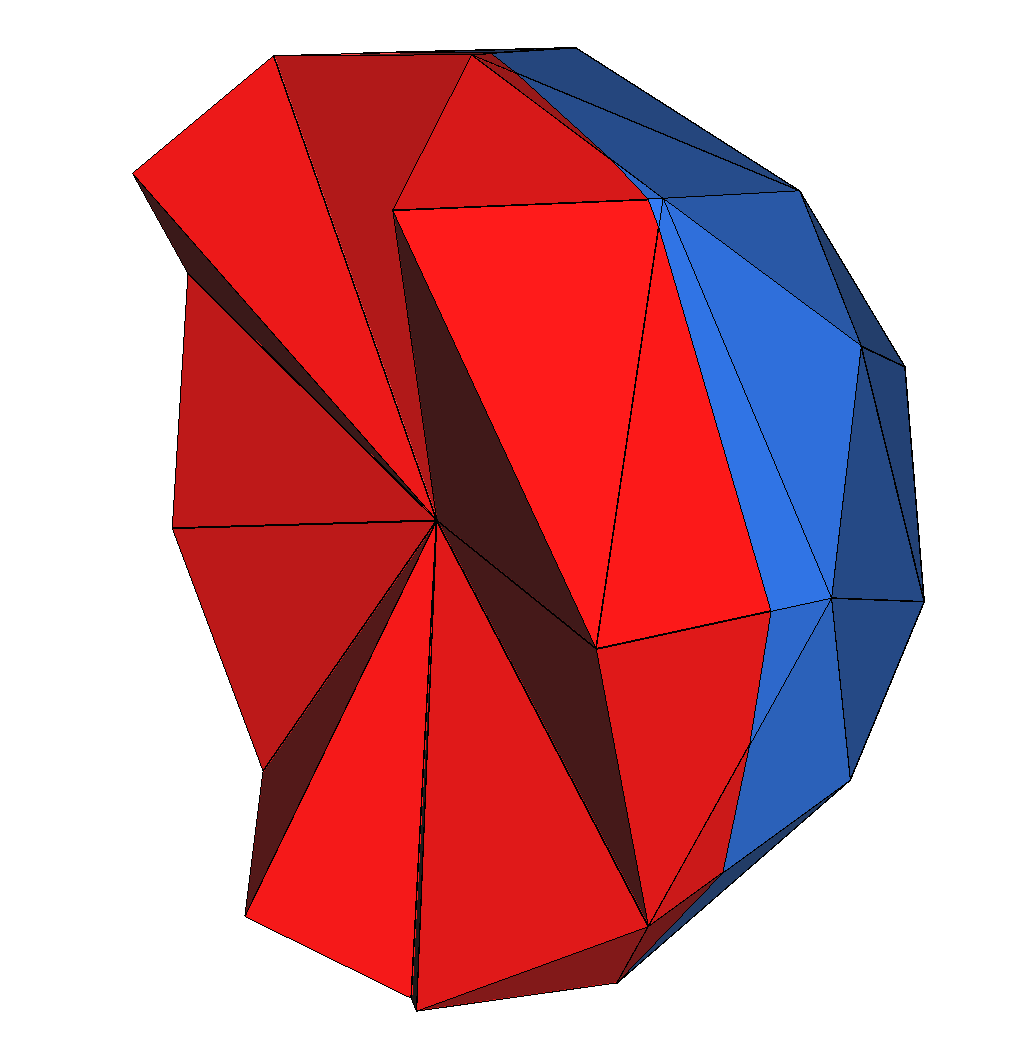
\includegraphics[height=5cm]{Mesh_3/pictures/implicit_domain_3}
   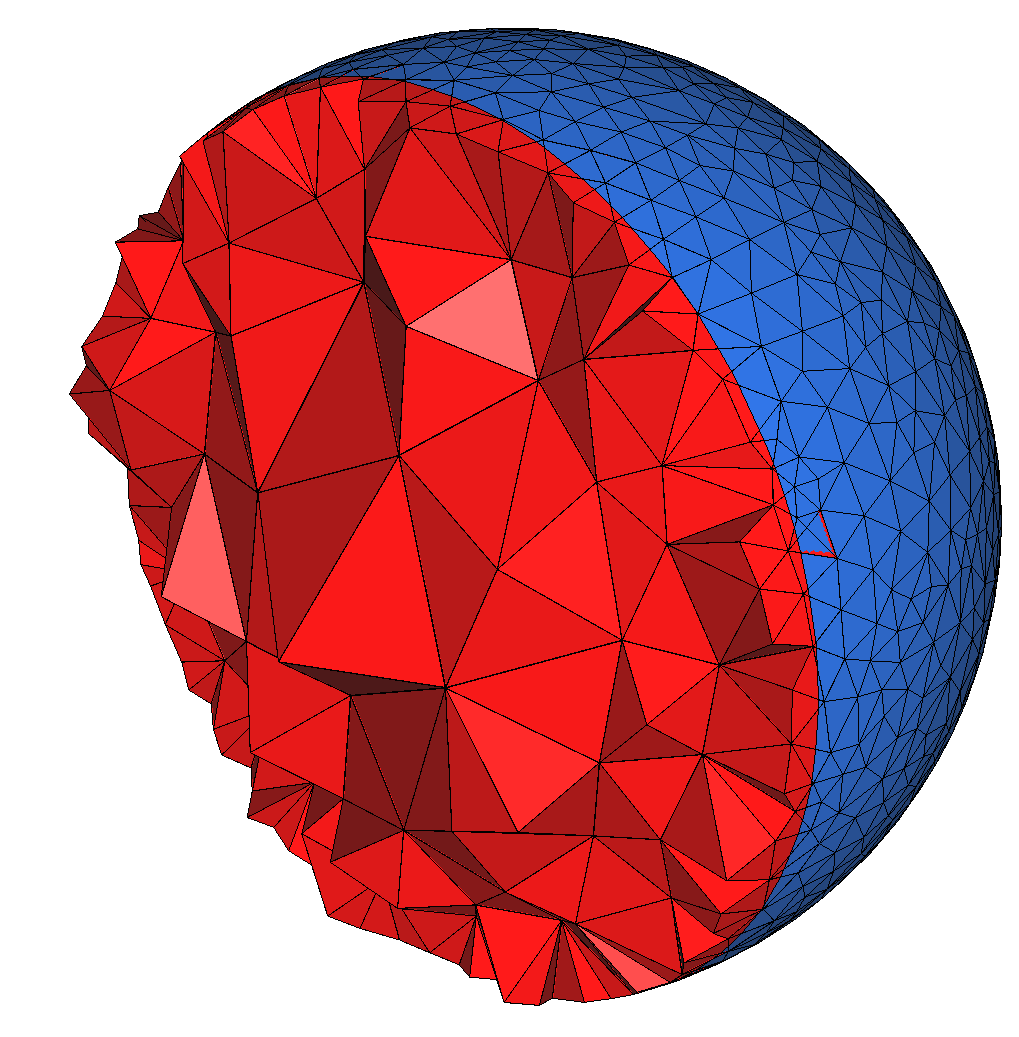
\includegraphics[height=5cm]{Mesh_3/pictures/implicit_domain_4}
   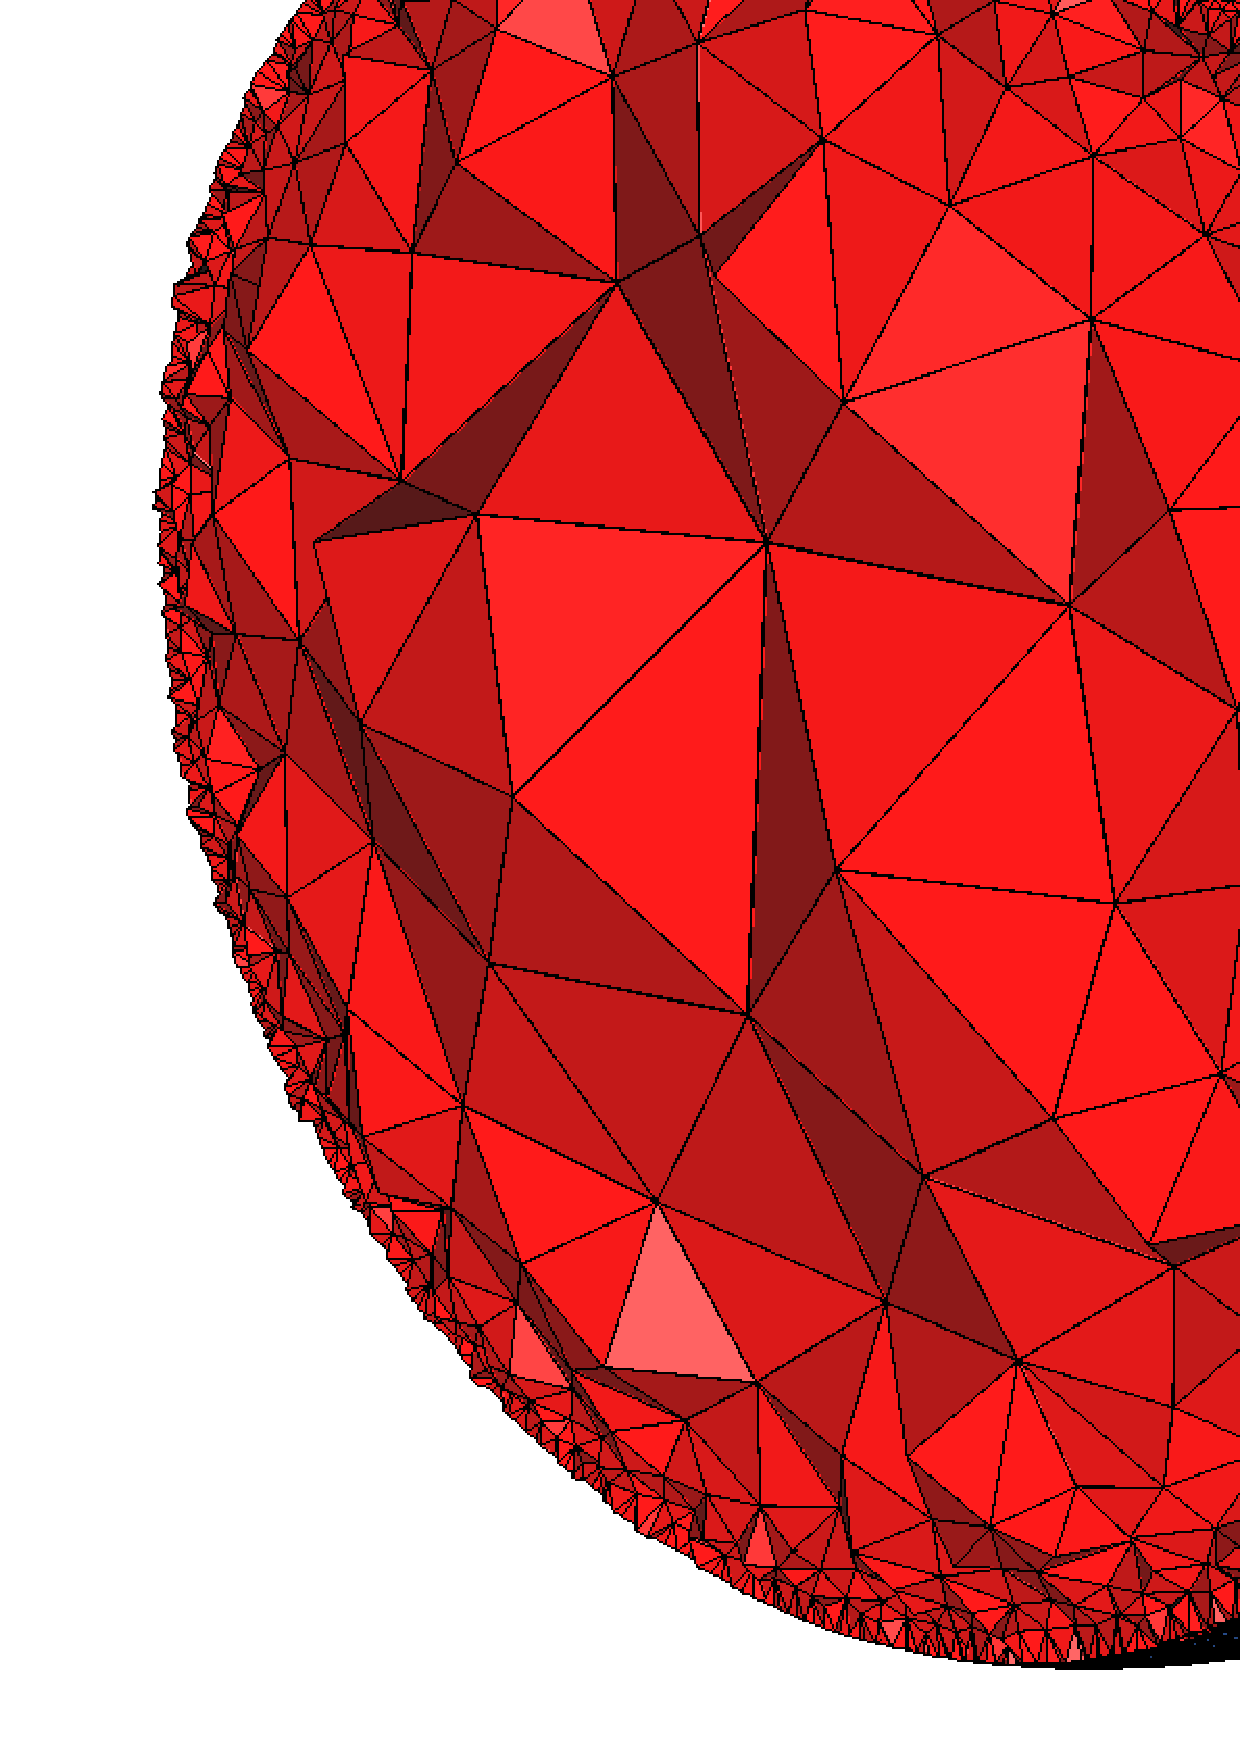
\includegraphics[height=5cm]{Mesh_3/pictures/implicit_domain_5}
 \end{ccTexOnly}
 \begin{ccHtmlOnly}
   <img border="0" height="250px" src="./pictures/implicit_domain.jpg"><br/>
   <img border="0" height="250px" src="./pictures/implicit_domain_3.jpg">
   <img border="0" height="250px" src="./pictures/implicit_domain_4.jpg">
   <img border="0" height="250px" src="./pictures/implicit_domain_5.jpg"><br/>
 \end{ccHtmlOnly}
 \caption{Top : the mesh  is obtained using the parameters $(25,0.15,0.05)$ for the angular bound,
radius bound and distance bound of  surface facets
and 
$(4,0.2)$ for  the radius-edge bound and radius  bound of mesh cells. The result is a  uniform mesh which contains tetrahedra
of about the same size. 
Bottom  left :
the mesh  is obtained by relaxing the \emph{ size bound} of tetrahedra
and facets.
 The result is a small coarse mesh. 
Bottom middle : the mesh  is obtained from the previous one  by tightening the \emph{distance bound} 
of surface facets to
$0.01$. The result is then a graded 3D mesh with a dense surface mesh
achieving a precise approximation. 
Bottom right :
the mesh  is obtained from the previous one  by fixing \emph{radius bound} of surface facets to $0.01$. The surface mesh is then denser to achieve the size bound.}
  \label{figure:parameters}
\end{center}
\end{figure}


If the domain has $1$-dimensional exposed features, the \ccc{criteria} includes
a sizing field to guide 
the sampling of $1$-dimensional features with  protecting balls centers.
%The criterion for $1$-dimensional features includes:\\
\begin{itemize}
\item \emph{\ccc{edge_size}}. This  constant or variable scalar field is used as an upper bound for the distance between two 
protecting ball centers  that are consecutive on a $1$-feature.
% \item \emph{a distance field}. This fields provides  an upper bound for the distance between any point on the
% segment joining two consecutive centers on a $1$-feature and the feature.
\end{itemize}

\subsubsection{The optimization parameters}

The   four  additional parameters  are optimization parameters.
They control which optimization processes are performed
and allow the user  to tune the parameters of the activated  optimization processes.
These parameters have internal types which are not described
but the library provides  global functions  to generate
appropriate values of these types:
\begin{itemize}
\item \ccc{parameters::lloyd()} and \ccc{parameters::no_lloyd()} activate and deactivate  the Lloyd smoother.
 \item \ccc{parameters::odt()} and \ccc{parameters::no_odt()} activate and deactivate the odt-smoother.
\item \ccc{parameters::perturb()} and \ccc{parameters::no_perturb()} activate and deactivate the perturber.
\item \ccc{parameters::exude()} and \ccc{parameters::no_exude()} activate and deactivate the exuder.
\end{itemize}


These parameters are optional and can be passed in any order.
If one parameter is not passed the default value is used. By default,
only the perturber and the exuder are activated.
Note that whatever may be the optimization processes activated by \ccc{make_mesh_3}
or \ccc{refine_mesh_3},
they are always launched in the order that is a suborder 
of the following:
\ccc{odt smoother}, \ccc{Lloyd smoother}, \ccc{perturber} and 
\ccc{exuder}. 

The package also provides four global functions to launch
each optimization process independently. These functions are useful for advanced experimentation 
on the efficiency of each optimization method.
Note however that the exuder adds on mesh vertices  weights that are conditioned by vertices
positions. 
Therefore an exudation process should never be run before
a smoother or a perturber. 
For a maximum efficiency, whatever  may be the optimization processes activated,
they should be launched in the order that is a suborder 
of the following:
\ccc{odt-smoother}, \ccc{Lloyd-smoother}, \ccc{perturber},
\ccc{exuder}. 

\ccSetThreeColumns{Mesh_optimization_return_code}{lloyd_optimize_mesh_3(C3T3& c3t3, MeshDomain_3 domain)}{}
\ccGlobalFunction{
	template< class C3T3, class MeshDomain_3 >
	Mesh_optimization_return_code lloyd_optimize_mesh_3(C3T3& c3t3, MeshDomain_3 domain);}{}
%, double time_limit=0, double sliver_bound=0,
%	int max_iteration_nb=0, double? convergence=0)
%\ccGlue
\ccGlobalFunction{
	template< class C3T3, class MeshDomain_3 >
	Mesh_optimization_return_code odt_optimize_mesh_3(C3T3& c3t3, MeshDomain_3 domain);}{}
%, double time_limit=0, double sliver_bound=0,
%	int max_iteration_nb=0, double? convergence=0
%\ccGlue
\ccGlobalFunction{
	template< class C3T3, class MeshDomain_3 >
	Mesh_optimization_return_code perturb_mesh_3(C3T3& c3t3, MeshDomain_3 domain);}{}
%, double time_limit=0, double sliver_bound=0
%\ccGlue
\ccGlobalFunction{
	template< class C3T3 >
	Mesh_optimization_return_code exude_mesh_3(C3T3& c3t3);}{}
%, double time_limit=0, double sliver_bound=0

Note that the global functions activating the optimization processes or launching
those processes have themselves parameters (see details in reference pages) to tune the optimization process.

\section{Examples}
\label{Mesh_3_section_examples}


\subsection{3D Domains Bounded by Isosurfaces}
The following code produces a 3D mesh for a domain whose boundary surface
is an  isosurface   defined by an implicit
function. Figure~\ref{figure:implicit_domain} shows a cut view of the
resulting mesh.

Note the use of named parameters (from Boost library) in the
constructor of the \ccc{Mesh_criteria} instance.

\ccIncludeExampleCode{Mesh_3/mesh_implicit_sphere.cpp}

\begin{figure}[ht]
\begin{center}
 \begin{ccTexOnly}
   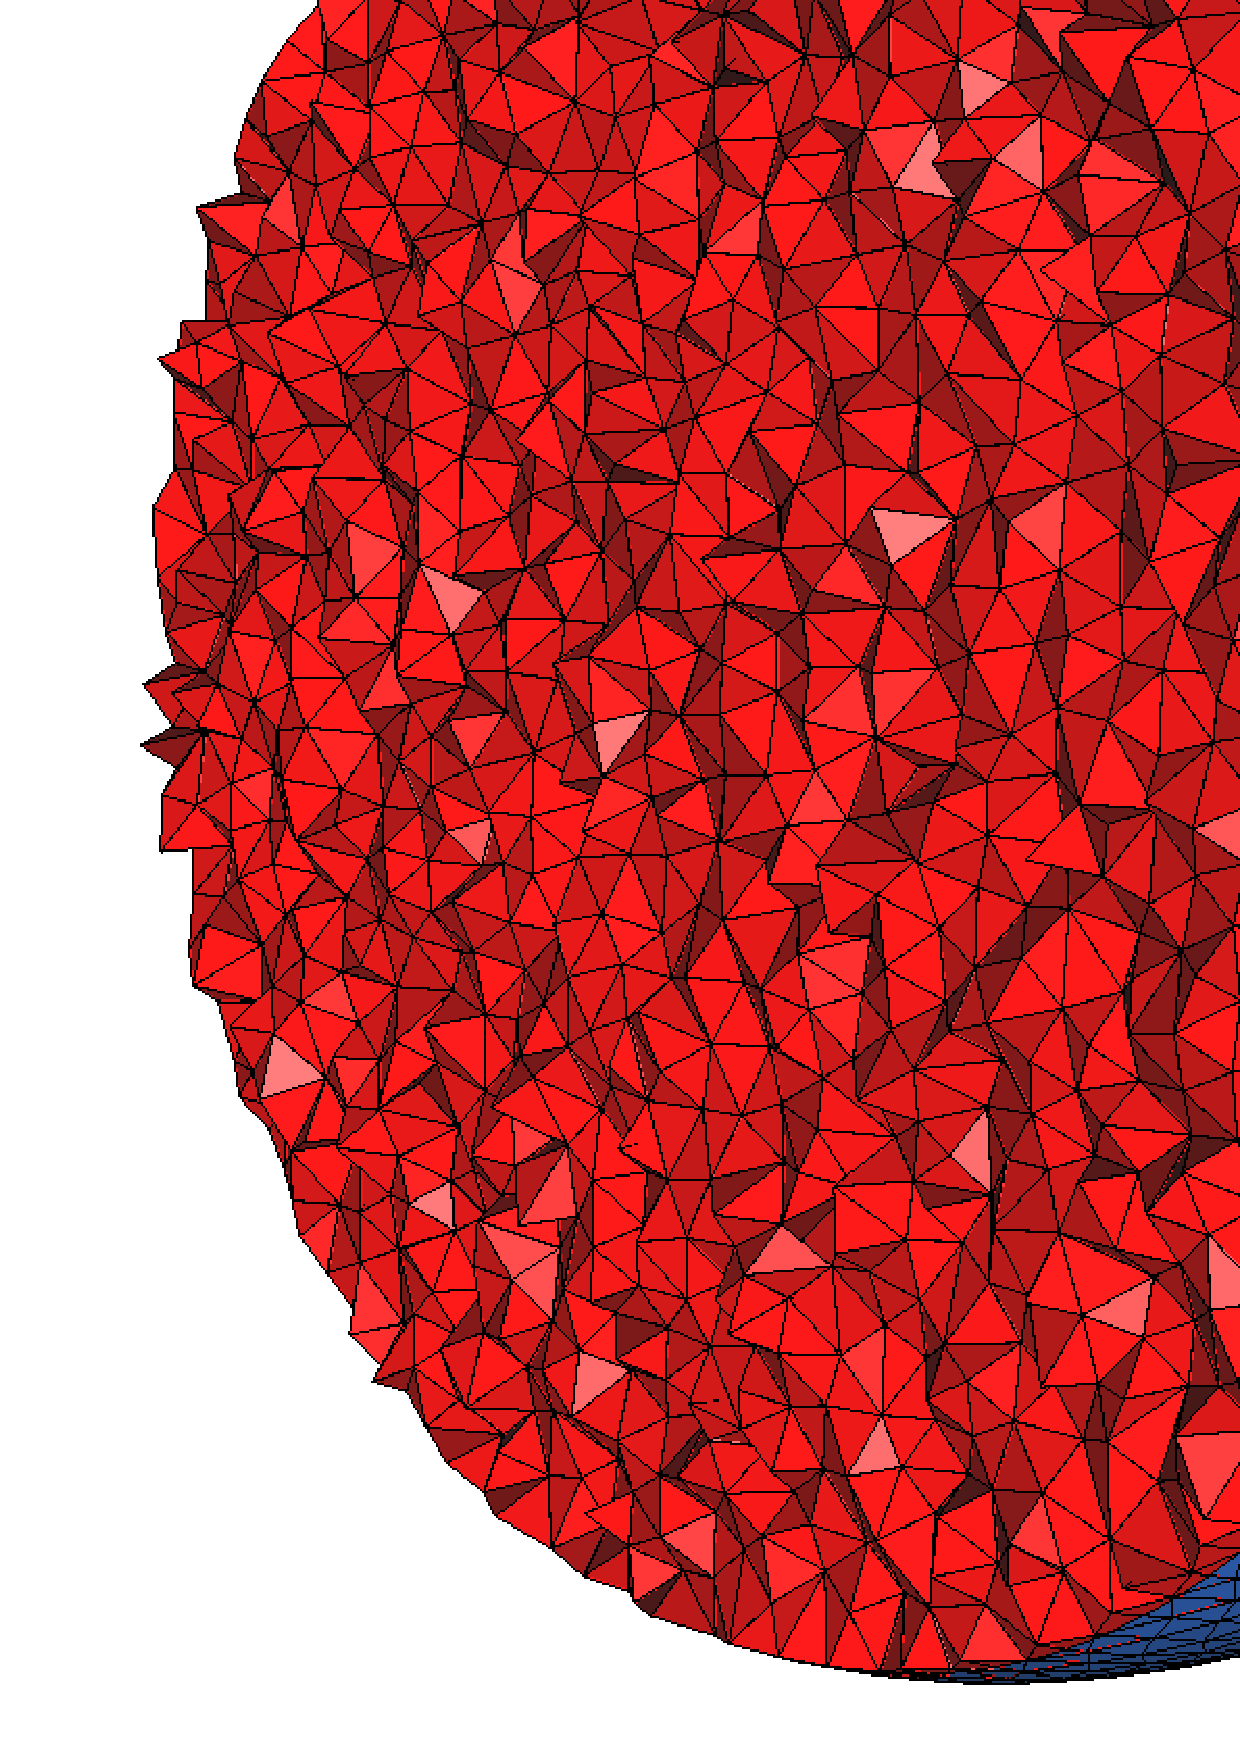
\includegraphics[height=6cm]{Mesh_3/pictures/implicit_domain}
 \end{ccTexOnly}
 \begin{ccHtmlOnly}
   <img border="0" src="./pictures/implicit_domain.jpg"><br/>
 \end{ccHtmlOnly}
 \caption{Cut view of a 3D mesh produced from an implicit domain}
  \label{figure:implicit_domain}
\end{center}
\end{figure}


\subsection{3D Polyhedral Domains}
\label{Mesh_3_subsection_examples_polyhedral}
The following code produces a 3D mesh for a domain
defined by polyhedral surfaces. Figure~\ref{figure:polyhedral_domain}
shows the resulting mesh.

\ccIncludeExampleCode{Mesh_3/mesh_polyhedral_domain.cpp}

\begin{figure}[ht]
\begin{center}
 \begin{ccTexOnly}
   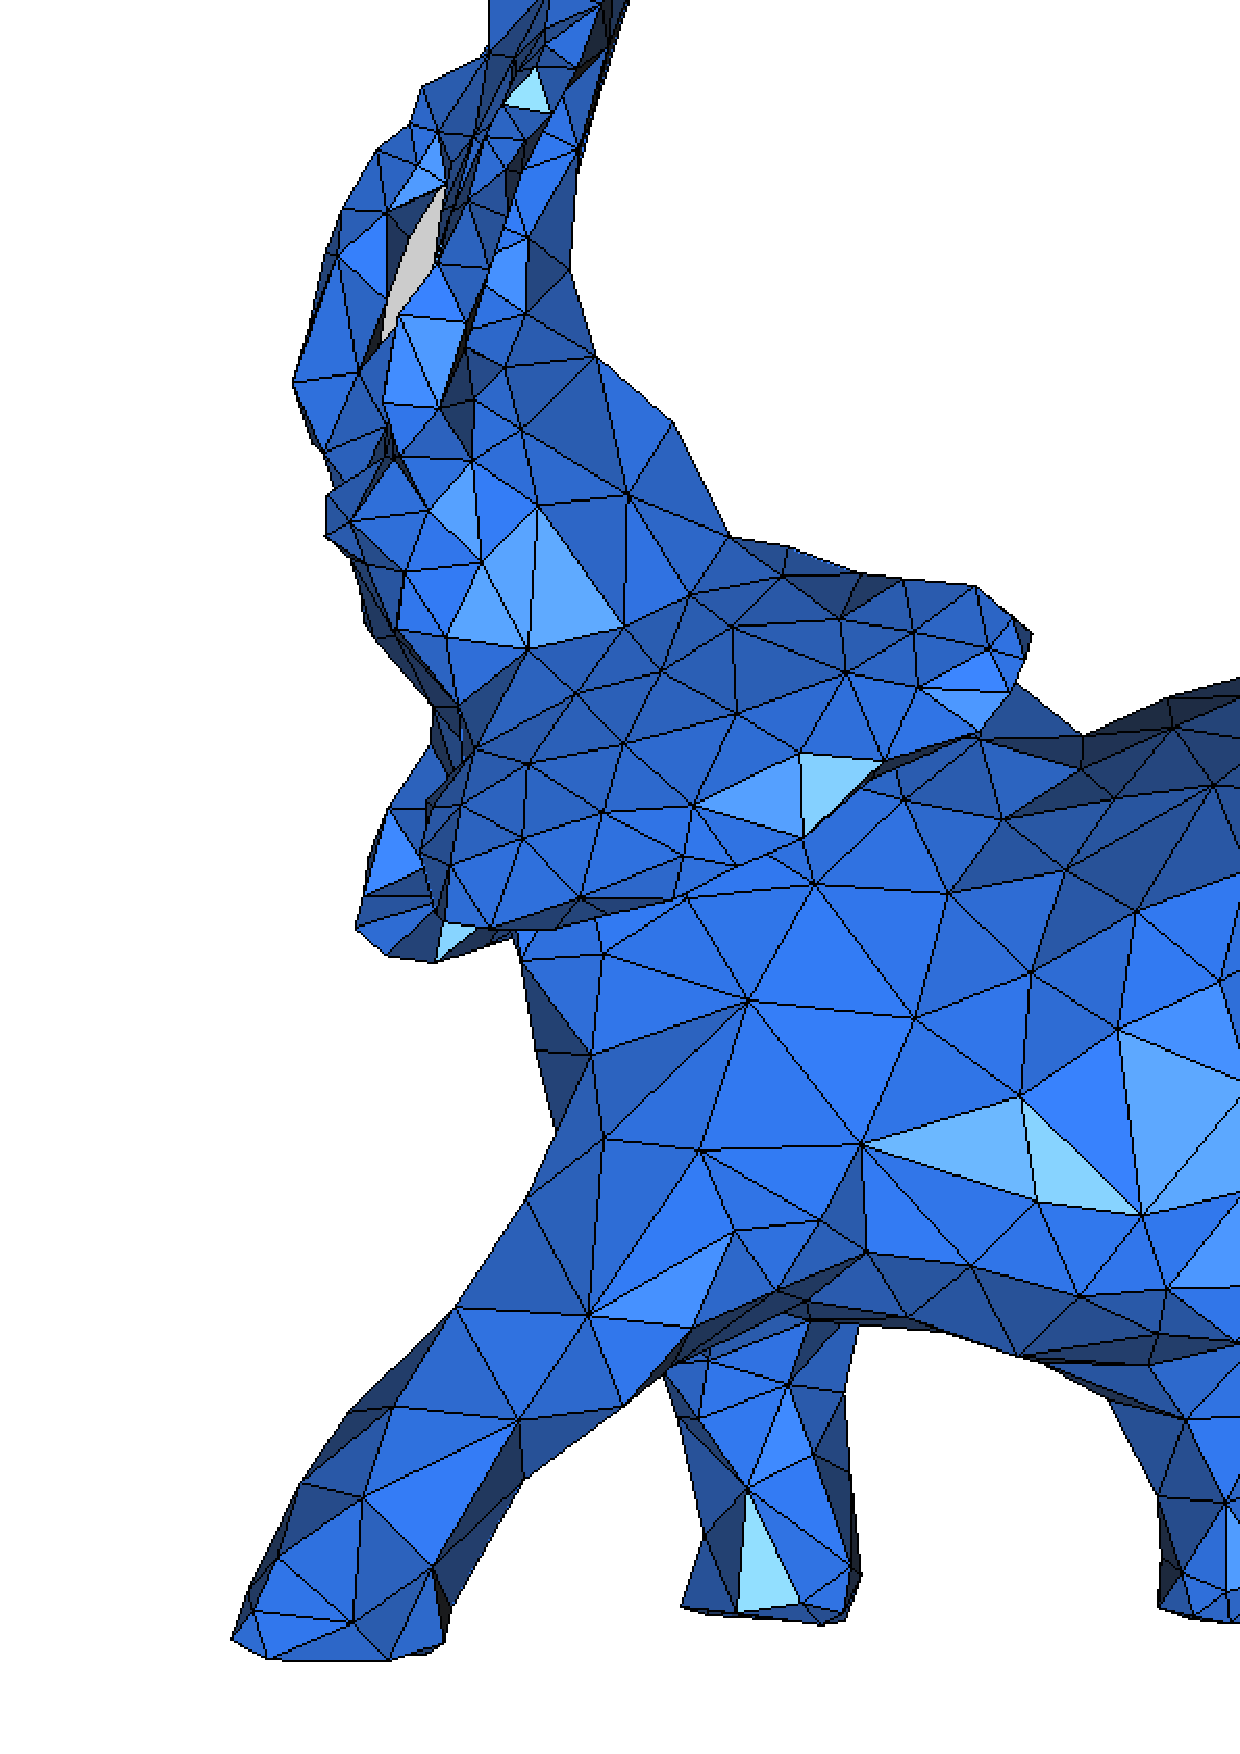
\includegraphics[height=7cm]{Mesh_3/pictures/polyhedral_domain}
   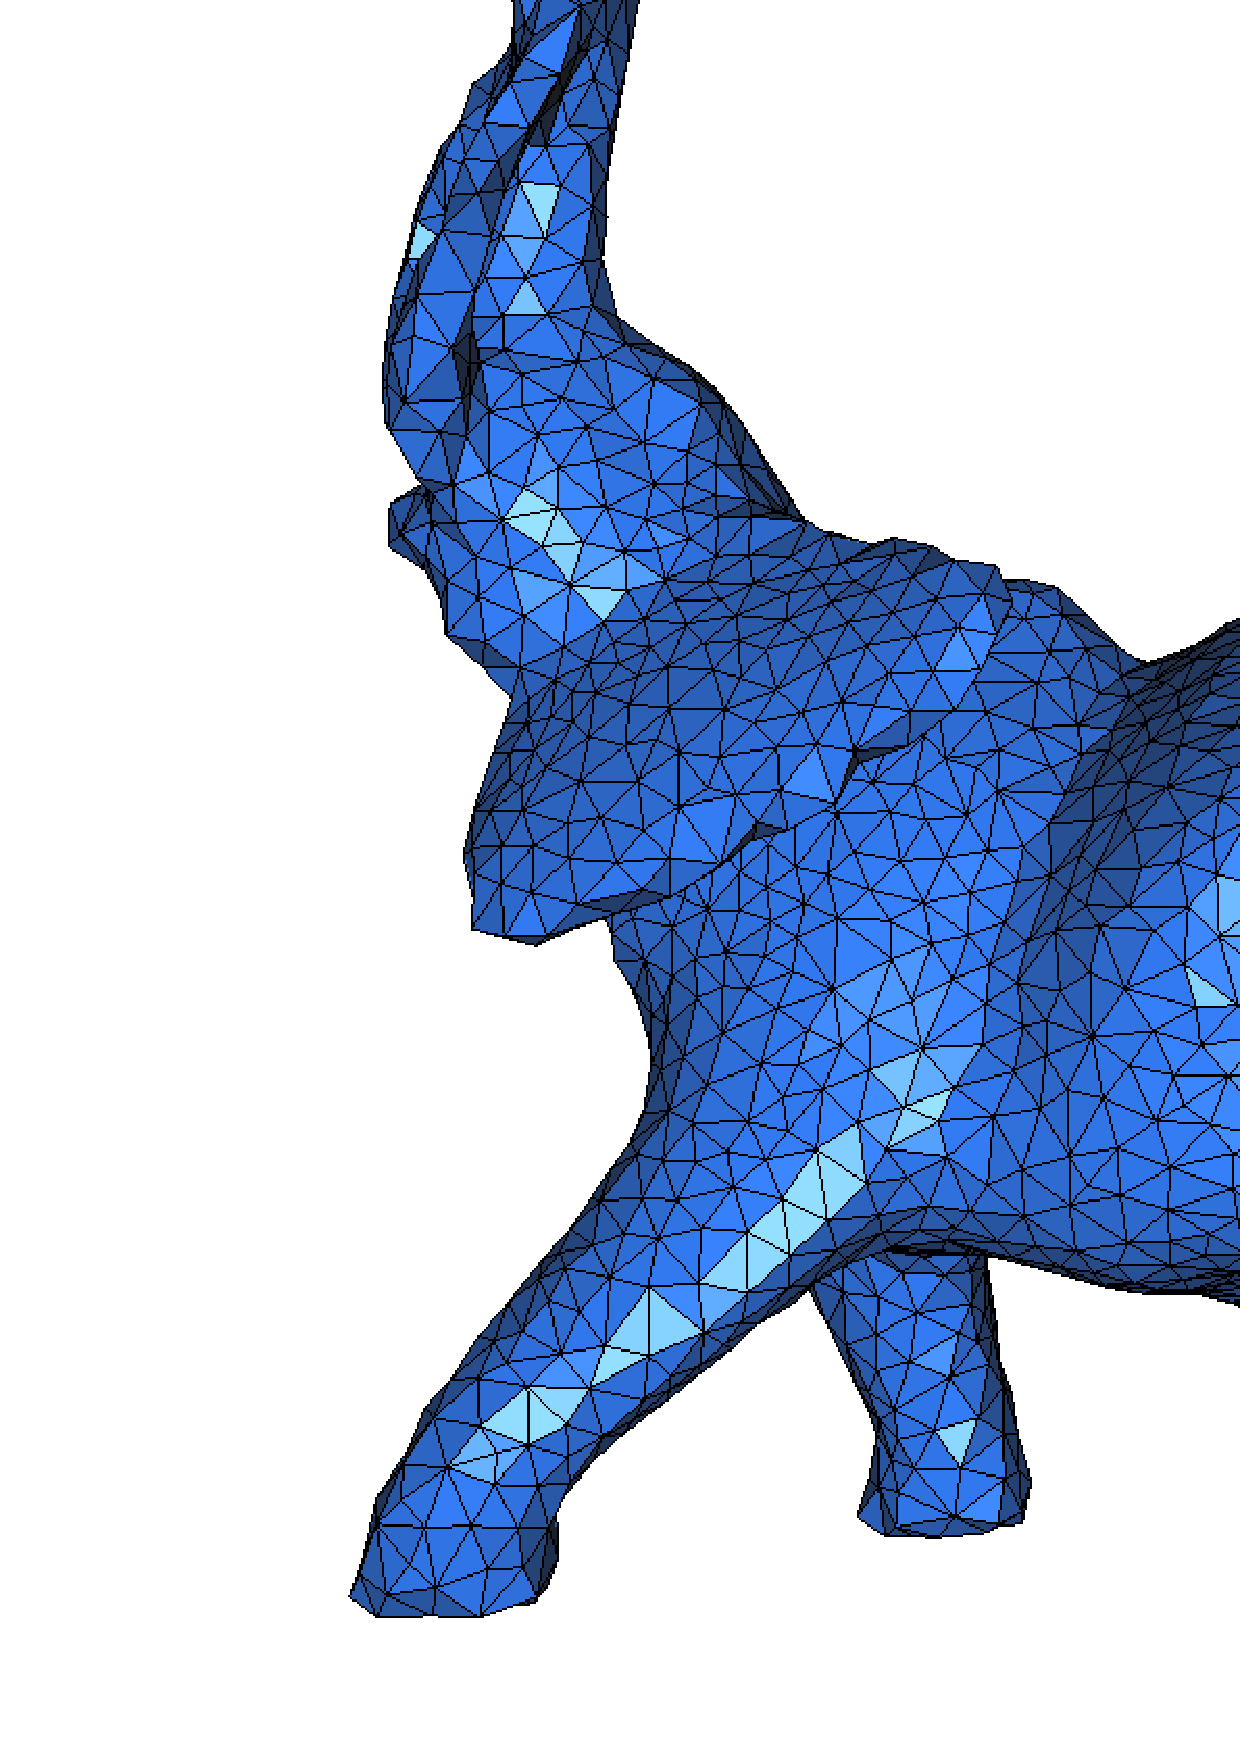
\includegraphics[height=7cm]{Mesh_3/pictures/polyhedral_domain_2}
 \end{ccTexOnly}
 \begin{ccHtmlOnly}
   <img border="0" src="./pictures/polyhedral_domain.jpg">
   <img border="0" src="./pictures/polyhedral_domain_2.jpg"><br/>
 \end{ccHtmlOnly}
 \caption{View of 3D meshes produced from a polyhedral domain. (i) 
   is a view of file out\_1.mesh and (ii) is a view of file
   out\_2.mesh. Code from
   subsection~\ref{Mesh_3_subsection_examples_polyhedral} generates
   these files.}
  \label{figure:polyhedral_domain}
\end{center}
\end{figure}


\subsection{Domains  From Segmented 3D Images}
\label{Mesh_3_subsection_examples_3d_image}
The following code produces  a 3D mesh from
a 3D image. The image is a segmented medical image  in which each 
voxel  is associated a label  in accordance with
the tissue  the voxel belongs to.
The domain is therefore a multi-domain
where each subdomain corresponds to a specific tissue.

In the following example, the image is read from the file
\ccc{liner.inr.gz} which is encoded in the format of the library Inrimage
\ccc{http://inrimage.gforge.inria.fr/}.
The resulting mesh is shown in Figure~\ref{figure:liver_3d_image_mesh}.

\ccIncludeExampleCode{Mesh_3/mesh_3D_image.cpp}

\begin{figure}[ht]
\begin{center}
 \begin{ccTexOnly}
   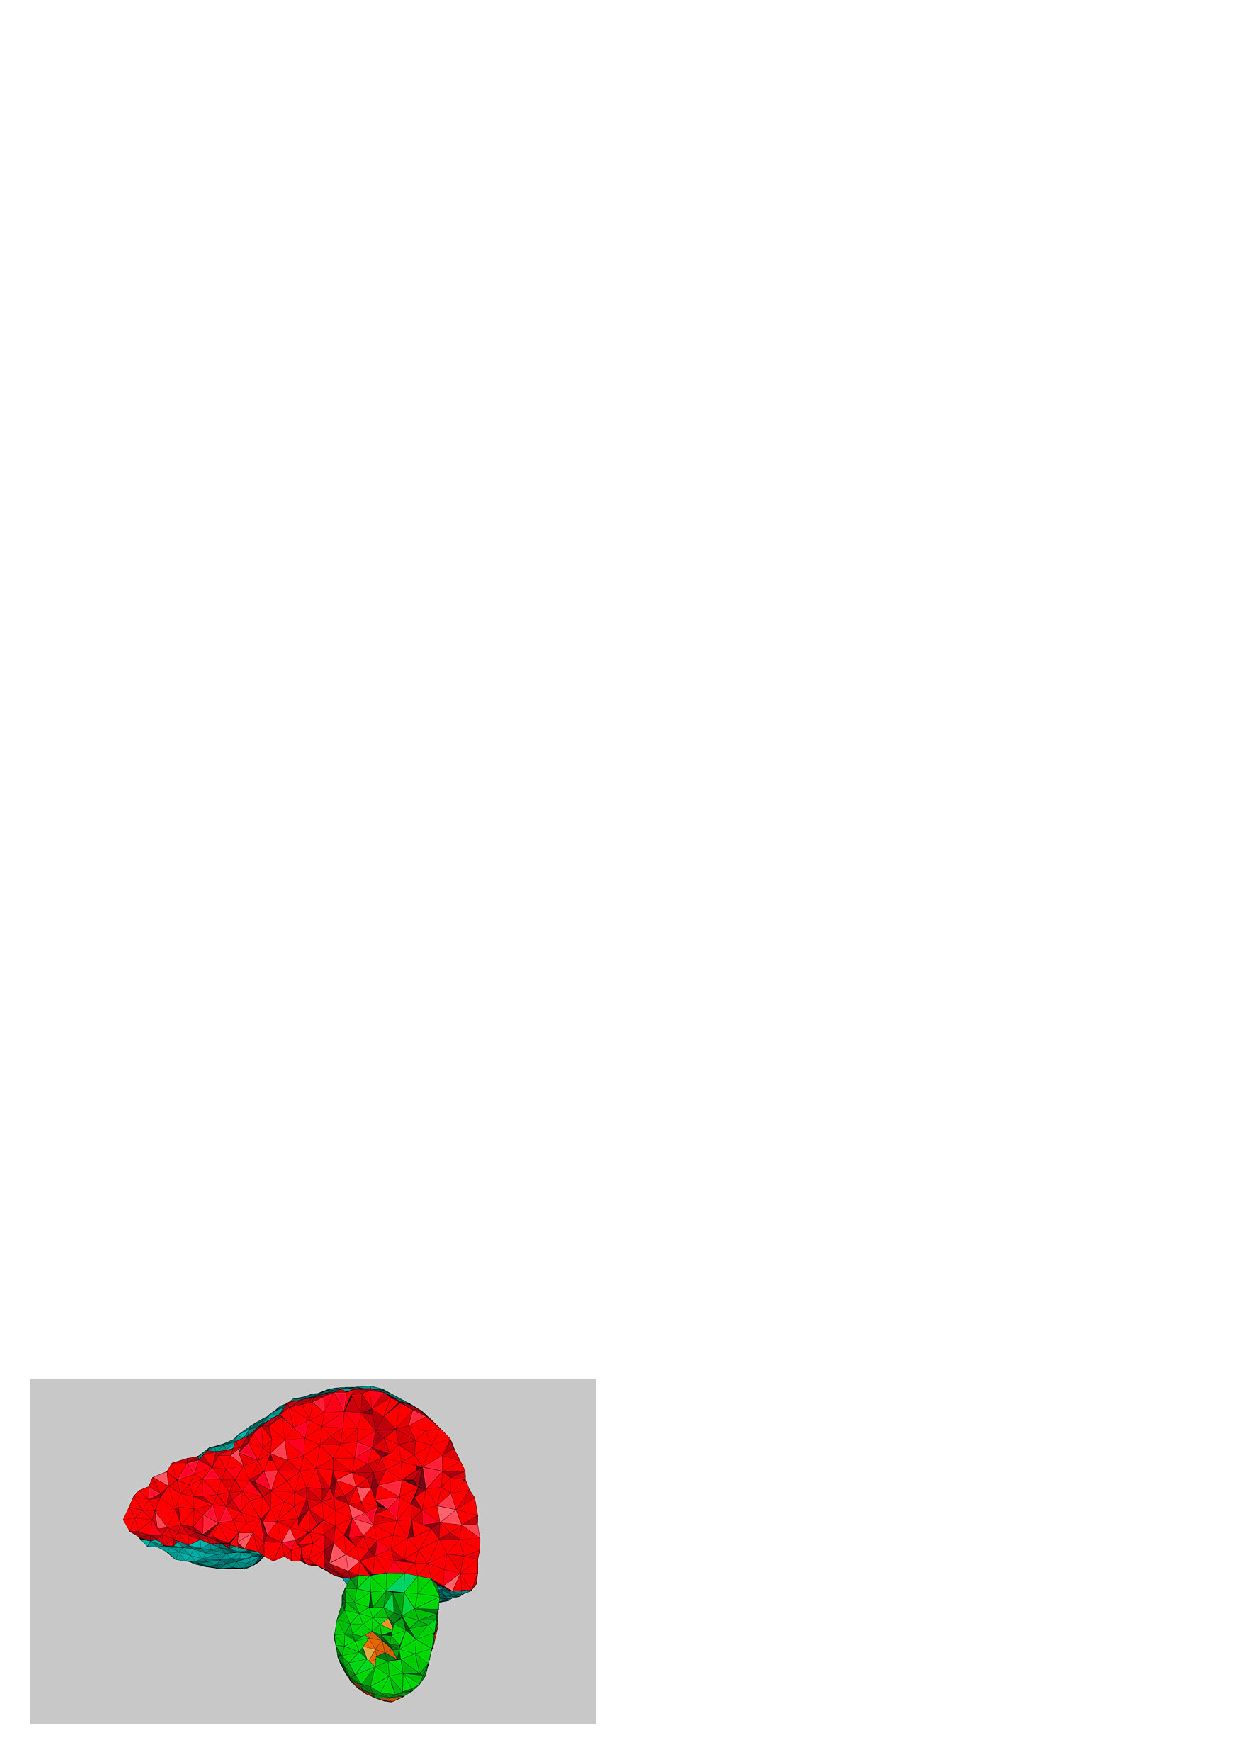
\includegraphics[width=10cm]{Mesh_3/pictures/liver}
 \end{ccTexOnly}
 \begin{ccHtmlOnly}
   <img border="0" src="./pictures/liver.jpg"><br/>
 \end{ccHtmlOnly}
 \caption{Cut view of a 3D mesh produced from a segmented liver image. Code from
 subsection~\ref{Mesh_3_subsection_examples_3d_image} generates this file.}
  \label{figure:liver_3d_image_mesh}
\end{center}
\end{figure}

\subsection{Using Variable Sizing Field}

\subsubsection{Sizing field as an analytical function}
\label{Mesh_3_subsubsection_examples_sphere_variable}

The following example shows how to use an analytical function as sizing field.

\ccIncludeExampleCode{Mesh_3/mesh_implicit_sphere_variable_size.cpp}

\begin{figure}[ht]
\begin{center}
 \begin{ccTexOnly}
   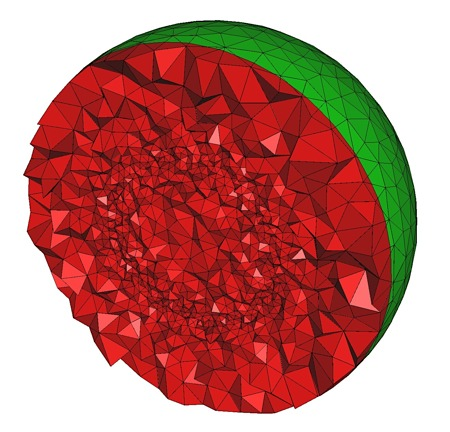
\includegraphics[width=7cm]{Mesh_3/pictures/sphere_variable}
 \end{ccTexOnly}
 \begin{ccHtmlOnly}
   <img border="0" src="./pictures/sphere_variable.jpg"><br/>
 \end{ccHtmlOnly}
 \caption{Cut view of a 3D mesh produced from an implicit sphere with non-constant
 sizing field. Code from
 subsection~\ref{Mesh_3_subsubsection_examples_sphere_variable} generates this file.}
  \label{figure:sphere_variable_mesh}
\end{center}
\end{figure}

\subsubsection{Different Sizing Field for Different Subdomains}
\label{Mesh_3_subsubsection_examples_3d_image_variable}

The following example shows how to use different size for different organs in
a 3D medical image.

\ccIncludeExampleCode{Mesh_3/mesh_3D_image_variable_size.cpp}

\begin{figure}[ht]
\begin{center}
 \begin{ccTexOnly}
   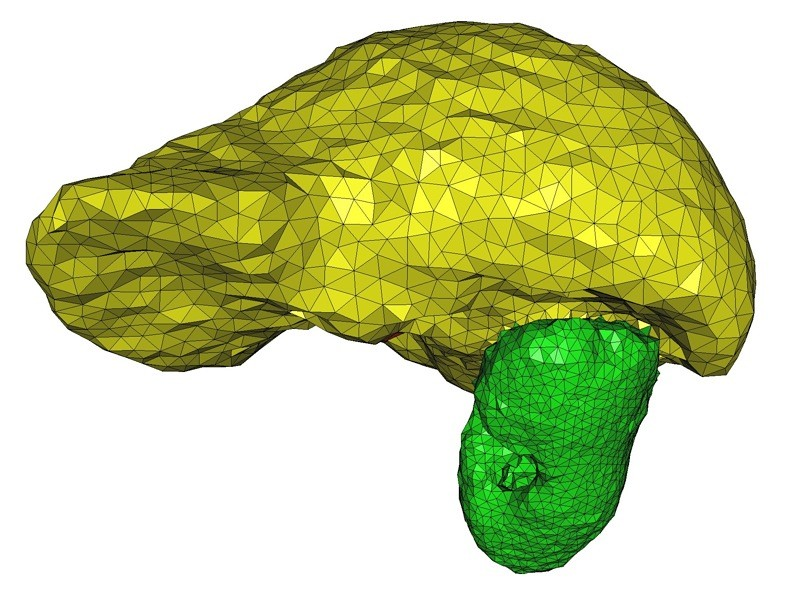
\includegraphics[width=9cm]{Mesh_3/pictures/liver_variable}
 \end{ccTexOnly}
 \begin{ccHtmlOnly}
   <img border="0" src="./pictures/liver_variable.jpg"><br/>
 \end{ccHtmlOnly}
 \caption{View of a 3D mesh produced from a 3D image with different size for
 different organs. Code from
 subsection~\ref{Mesh_3_subsubsection_examples_3d_image_variable} generates this file.}
  \label{figure:liver_variable_mesh}
\end{center}
\end{figure}


\subsection{Meshing Domains with Sharp Features}
\label{Mesh_3_subsection_example_polyhedral_with_edges}

\subsubsection{3D polyhedral domain with edges }
The following example shows how to generate a mesh from a polyhedral
surface. The output mesh conforms to the sharp features of the input surface.

\ccIncludeExampleCode{Mesh_3/mesh_polyhedral_domain_with_features.cpp}

\begin{figure}[ht]
\begin{center}
 \begin{ccTexOnly}
   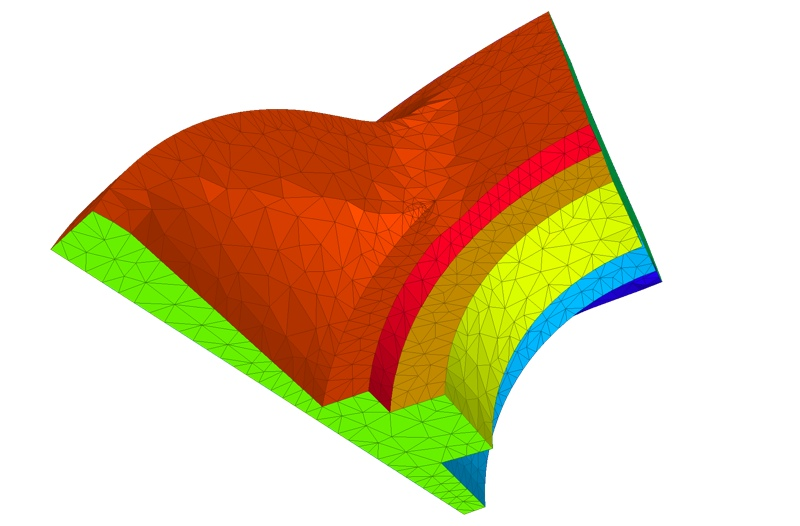
\includegraphics[width=10cm]{Mesh_3/pictures/fandisk}
 \end{ccTexOnly}
 \begin{ccHtmlOnly}
   <img border="0" src="./pictures/fandisk.jpg"><br/>
 \end{ccHtmlOnly}
 \caption{View of a 3D mesh with sharp features. Code from
 subsection~\ref{Mesh_3_subsection_example_polyhedral_with_edges} generates this mesh.}
  \label{figure:fandisk_mesh}
\end{center}
\end{figure}


\subsubsection{Implicit domain with 1D features}
The following example shows how to generate a mesh from an implicit
domain. We add by hand the intersection of the spheres as a sharp feature. 

\ccIncludeExampleCode{Mesh_3/mesh_two_implicit_spheres_with_balls.cpp}

\begin{figure}[ht]
\begin{center}
 \begin{ccTexOnly}
   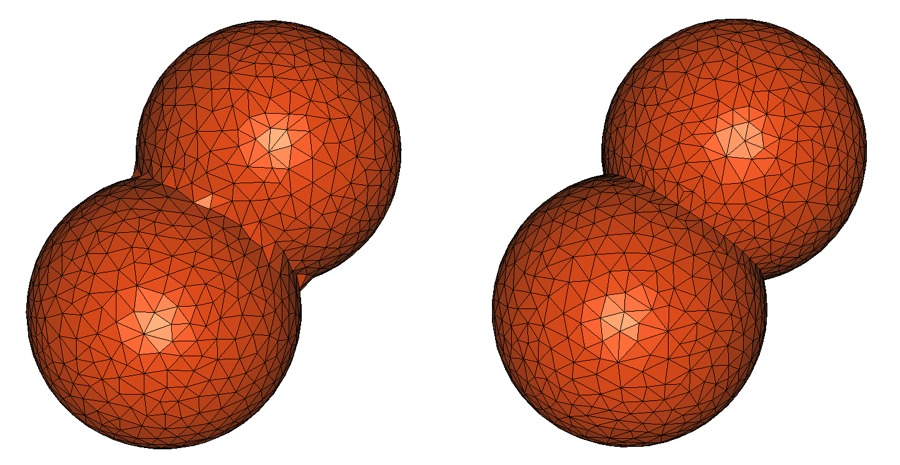
\includegraphics[width=12cm]{Mesh_3/pictures/twospheres}
 \end{ccTexOnly}
 \begin{ccHtmlOnly}
   <img border="0" src="./pictures/twospheres.jpg"><br/>
 \end{ccHtmlOnly}
 \caption{View of a 3D mesh with sharp features generated from two intersected
 implicit spheres. On the left, one can see the mesh without feature preservation,
 and on the right the mesh with feature preservation.}
  \label{figure:two_spheres_mesh}
\end{center}
\end{figure}


\subsection{Tuning Mesh Optimization}
\label{Mesh_3_subsection_examples_optimization}

In the previous examples, the mesh generation is launched through a  call
\ccc{make_mesh_3(domain,criteria)} with a minimal number of parameters. In such cases, 
the default optimization strategy is applied: after the Delaunay refinement process
 two optimization steps are performed, a perturbation and  a sliver exudation.
The following examples show how to disable default optimization steps 
and how to tune the parameters of optimization steps.



\subsubsection{Disabling exudation and tuning perturbation}

In this first example, we show how to disable the exudation step.
The optimization phase after the refinement includes only
a perturbation phase which is launched  with no time bound
and an objective of 10 degrees for the minimum dihedral angle
of the mesh.
The example shows two ways of achieving the same result. The first way
issues a single call to \ccc{make_mesh_3} with the required optimization 
process activated and tuned. In the second way, \ccc{make_mesh_3} is first called
without any optimization process and the resulting mesh is next optimized
through a call to \ccc{perturb_mesh_3} with tuned parameters.

\ccIncludeExampleCode{Mesh_3/mesh_optimization_example.cpp}


\subsubsection{Using Lloyd global optimization}

In this second example, we show how to call  the Lloyd optimization on the
mesh, followed by a call to exudation. We set a time bound of 30s for the Lloyd optimization. 
We set a time bound of 10s and a sliver bound of 10 degrees for the exuder.

\ccIncludeExampleCode{Mesh_3/mesh_optimization_lloyd_example.cpp}





\section{Performances}

We provide here some benchmarks of the performances of the mesh generation engine. The machine
used is a PC running Linux64 with two Intel Xeon CPU X5450 clocked at 3.00 GHz
with 32GB of RAM. The program has been compiled with g++ v4.3.2 with the -O3 option. 
Note that our implementation does not take advantage of multi-core
architectures.

Those benchmarks have been done using \cgal\ v3.8.

\subsection{Delaunay refinement}

We study the refinement part of the mesh generation engine in this section. We
give the CPU time (measured by \ccc{CGAL::Timer}) using the 3 provided oracles. In all experiments, we produce well
shaped elements: we set the facet angle bound and the radius edge bound to their
theoretical limit (resp. 30 degrees and 2). We also use the same uniform sizing field for facets
and cells.

\subsubsection{Implicit function}

We mesh an analytical sphere of radius 1.

\begin{center}
\begin{tabular}{|l|l|l|l||c|c|}
  \hline
  Size bound & vertices nb & facets nb & tetrahedra nb & CPU Time (s) & vertices/second\\
  \hline
  0.2 & 499 & 488 & 2,299 & 0.0240 & 20,800 \\
  0.1 & 3,480 & 2,046 & 18,756 & 0.146 & 23,800 \\
  0.05 & 25,556 & 8,274 & 149,703 & 1.50 & 17,000 \\
  0.025 & 195,506 & 33,212 & 1,194,727 & 17.4 & 11,200 \\
  0.0125 & 1,528,636 & 134,810 & 9,547,772 & 179 & 8,530 \\
  \hline
\end{tabular}
\end{center}

\subsubsection{Polyhedral domain}

\begin{figure}[ht]
\begin{center}
 \begin{ccTexOnly}
   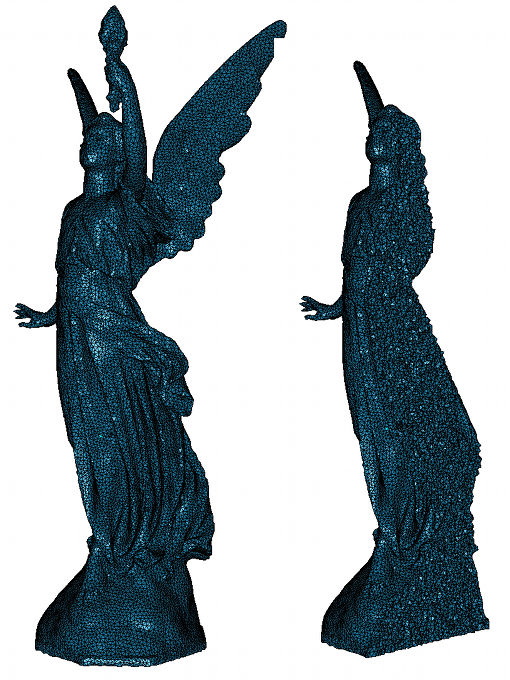
\includegraphics[width=10cm]{Mesh_3/pictures/bench_polyhedral.jpg}
 \end{ccTexOnly}
 \begin{ccHtmlOnly}
   <img border="0" src="./pictures/bench_polyhedral.jpg"><br/>
 \end{ccHtmlOnly}
 \caption{View of polyhedral mesh generation result (size = 0.005).}
  \label{figure:mesh_3_benchmark_polyhedral}
\end{center}
\end{figure}

We mesh a volume bounded by a closed triangulated surface made of about 50,000 vertices and 100,000 triangles.
Picture~\ref{figure:mesh_3_benchmark_polyhedral} shows the mesh obtained when
size is set to 0.005.

\begin{center}
\begin{tabular}{|l|l|l|l||c|c|}
  \hline
  Size bound & vertices nb & facets nb & tetrahedra nb & CPU Time (s) & vertices/second \\
  \hline
  0.04 & 423 & 717 & 1,332 & 0.488 & 866 \\
  0.02 & 2,638 & 3,414 & 10,957 & 2.64 & 998 \\
  0.01 & 18,168 & 15,576 & 90,338 & 13.9 & 1,310 \\
  0.005 & 129,442 & 64,645 & 722,018 & 66.7 & 1,940 \\
  0.0025 & 967,402 & 263,720 & 5,756,491 & 348 & 2,780 \\
  \hline
\end{tabular}
\end{center}

\subsubsection{3D image}

\begin{figure}[ht]
\begin{center}
 \begin{ccTexOnly}
   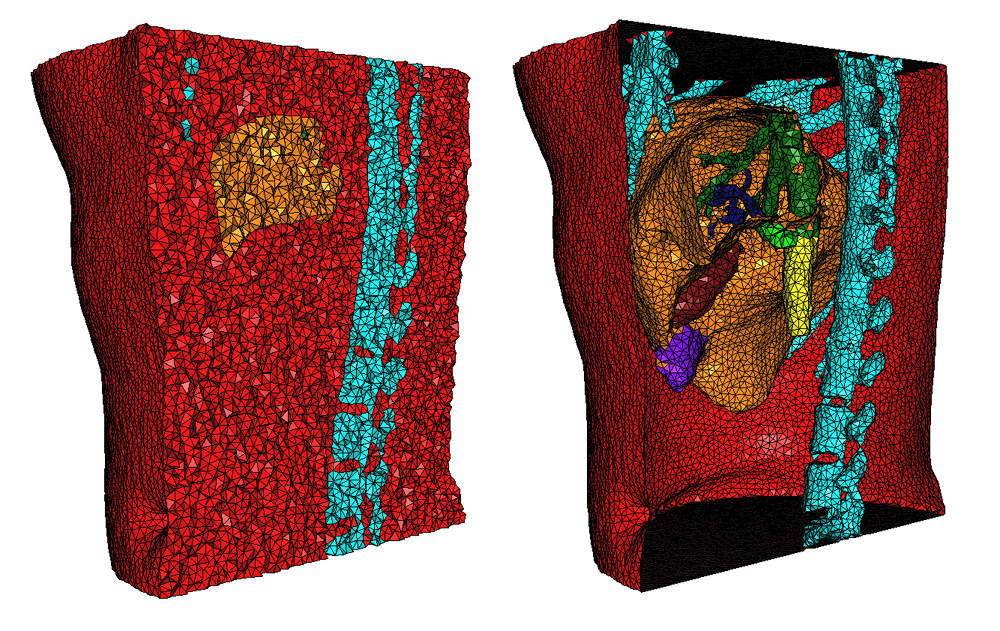
\includegraphics[width=14cm]{Mesh_3/pictures/bench_3d.jpg}
 \end{ccTexOnly}
 \begin{ccHtmlOnly}
   <img border="0" src="./pictures/bench_3d.jpg"><br/>
 \end{ccHtmlOnly}
 \caption{View of 3d image mesh generation result (size = 4).}
  \label{figure:mesh_3_benchmark_3d_image}
\end{center}
\end{figure}

We mesh image number 2 from the 3D-IRCADb-01\footnote{available at \lcTex{\url{http://www.ircad.fr/softwares/3Dircadb/3Dircadb1/index.php}} \lcRawHtml{<A href="http://www.ircad.fr/softwares/3Dircadb/3Dircadb1/index.php">http://www.ircad.fr/softwares/3Dircadb/3Dircadb1/index.php</A>}} public database.
The size of this image is 512x512x172 voxels (about 45M voxels). The size of the voxels
is 0.78mm x 0.78mm x 1.6mm. Picture~\ref{figure:mesh_3_benchmark_3d_image}
shows the mesh obtained for size set to 4.

\begin{center}
\begin{tabular}{|l|l|l|l||c|c|}
  \hline
  Size bound (mm) & vertices nb & facets nb & tetrahedra nb & CPU Time (s) & vertices/second\\
  \hline
  16 & 3,898 & 4,099 & 20,692 & 0.344 & 11,300 \\
  8 & 34,117 & 27,792 & 199,864 & 3.09 & 11,000 \\
  4 & 206,566 & 86,180 & 1,253,694 & 22.4 & 9,230 \\
  2 & 1,546,196 & 329,758 & 9,617,278 & 199 & 7,780 \\
  \hline
\end{tabular}
\end{center}

%\subsection{Mesh optimization}

%\subsubsection{Exudation}

\section{Design and Implementation History}


\subsubsection{Theoretical  foundations}


The \cgal\ mesh generation package implements a  meshing engine based 
on the method of   Delaunay refinement introduced by Chew~\cite{c-gqmgc-93}  and Ruppert~\cite{r-draq2d-95}
and pioneered in 3D by Shewchuk~\cite{s-tmgdr-98}. 
It uses the notion of restricted Delaunay triangulation
 to approximate $1$-dimensional curved features and  curved surface patches
and rely on the work of Boissonnat and Oudot~\cite{cgal:bo-pgsms-05}
and Oudot et al.~\cite{cgal:ory-mvbss-05}
to achieve accurate representation of boundary and subdividing surfaces in the mesh.
The mechanism of protecting balls, used to ensure a fair representation
of $1$-dimensional features, if any, and the termination of the refinement process
whatever may be the input geometry, in particular whatever small dihedral angles may form
the boundary and subdivision surface patches,
was pioneered by Cheng et al.~\cite{cgal:cdr-drpsc-07} and further experimented by Dey, Levine et al.
~\cite{cgal:cdl-pdma-07}.
The optimization phase involves global optimization processes, a perturbation process
and a sliver exudation process. The global optimizers are based on Lloyd smoothing~\cite{cgal:dfg-cvtaa-99t, cgal:dw-tmgob-02}
and odt smoothing~\cite{cgal::c-mssbo-04,cgal:acyd-vtm-05}, where odt means
\emph{optimal Delaunay triangulation}. The perturbation process 
is mainly based on the work of Tournois~\cite{cgal:t-om-09}
and Tournois et al.~\cite{cgal:twad-iropitmg-09},
while the exudation process is, the now famous,  optimization by weighting described
in Edelsbrunner et al.~\cite{cgal:cdeft-slive-00}.


\subsubsection{Implementation history}
Work on the package \ccc{Mesh_3} started during the PhD thesis of Laurent Rineau
advised by Mariette Yvinec.  A  code prototype, together
with a first version of design and specifications~\cite{cgal:ry-gsddrm-06}
came out of their collaboration.

From the beginning of 2009, most of the work has been performed by St\'ephane
Tayeb, in collaboration with Mariette Yvinec, Laurent Rineau, Pierre Alliez and Jane Tournois.
First, St\'ephane released the first public version of the package, implementing the specifications
written by Laurent and Mariette. 

The optimization processes are
heavily based on the work of Jane Tournois and Pierre Alliez
during the PhD of Jane advised by Pierre. The optimization phase was imported
in the mesh generation package by St\'ephane Tayeb
and appeared first in  release 3.6 of \cgal.

In collaboration with Laurent Rineau, St\'ephane also added demos and examples.
After some experiments on medical imaging data performed by
Dobrina Boltcheva et al.~\cite{cgal:byb-mgmmi-09, cgal:-byb-fpdmgmmi-09}, the handling
of $1$-dimensional features was worked out by Laurent Rineau, St\'ephane Tayeb
and Mariette Yvinec. It appeared first in the release 3.8  of \cgal.
 


